\documentclass[10pt]{article}

\usepackage[utf8]{inputenc}
\usepackage[francais]{babel}
\usepackage{multicol}
\usepackage{float}
\usepackage{tikz}

% FAMFAMFAM.com colors
\definecolor{mpink}{RGB}{255,11,91}
\definecolor{mblue}{RGB}{11,206,255}
\definecolor{mgreen}{RGB}{123,255,45}

\setlength{\textwidth}{39pc}
\setlength{\textheight}{50pc}
\setlength{\parindent}{1em}
\setlength{\parskip}{0pt plus 1pt}
\setlength{\oddsidemargin}{0pc}
\setlength{\marginparwidth}{0pc}
\setlength{\topmargin}{1pc}
\setlength{\headsep}{20pt}
\setlength{\columnsep}{2pc}

\title{Recherche décentralisée de connexité pour réseaux de capteurs mobiles}
\author{Merwan Achibet}
\date{}

\begin{document}

\maketitle

\begin{multicols}{2}

\section{Introduction}

On imagine le problème suivant : un groupe de $n$ capteurs mobiles est
réparti aléatoirement dans un espace aérien. On part de l'hypothèse
qu'un capteur connaît uniquement le nombre total de capteurs de ce
système et qu'il est assez sophistiqué pour pouvoir déterminer
précisément sa position absolue. Les capteurs sont dotés de matériel
de communication sans fil et peuvent s'envoyer des messages à
condition que la distance les séparant soit inférieure à un seuil
donné.

Le réseau constitué par cet essaim d'appareils volants forme un graphe
dynamique dont les n\oe uds sont les capteurs. Deux n\oe uds sont
reliés par un arc si les capteurs qui leur sont associés sont en
mesure de communiquer, id est s'ils sont assez proches. La figure
\ref{communication} illustre un scénario impliquant trois capteurs.

\begin{figure}[H]

  \centering

  \begin{tikzpicture}

  \draw (0,0) -- (-1,1);

  \drawSensor{0}{0}{2}{red}
  \drawSensor{-1}{1}{2}{blue}
  \drawSensor{2.5}{1}{2}{green}

\end{tikzpicture}


  \caption{Les capteurs rose et bleu peuvent communiquer et sont
    connectés tandis que le capteur vert est isolé.}
  \label{communication}

\end{figure}

On considère un capteur comme un agent autonome capable de se mouvoir
dans l'espace. Afin de ne pas se ??? de considérations géométriques
superflues, il est supposé qu'un capteur conserve toujours la même
altitude et donc qu'il évolue dans un espace euclidien de dimension
2. La contrainte principale de cet exercice est que l'on refuse toute
forme de contrôle global sur l'essaim de capteurs. Toutes les actions
entreprises par un appareil seront uniquement dû à ses décisions
propres; décisions dépendants de la vision réduite du système que sa
périphérie

La possibilité pour un capteur de communiquer avec ses semblables est
au centre de nos préoccupations car on considère qu'un capteur isolé
est inutile puiqu'incapable de transmettre des données.

Deux questions se posent :

\begin{enumerate}
\item{Comment déterminer si le réseau de capteurs est connexe ?}
\item{Comment guider les capteurs de façon à ce qu'il le devienne ?}
\end{enumerate}

\section{Déterminer si le réseau est connexe}

\section{Rendre le réseau connexe}

La résolution de ce problème passe par la satisfaction de deux besoins
a priori antagonistes. D'une part, il est naturellement nécessaire de
réunir les capteurs dans un espace réduit, de façon à ce qu'ils
puissent communiquer et échanger des données en continu. D'autre part,
et dans l'interêt de leurs utilisateurs, ils doivent s'étaler dans
l'espace afin d'effectuer des mesures sur la plus grande superficie
possible. Nous sommes donc dans une situation de compromis, dans
laquelle une contrainte technique (la portée de communication) force à
agglomérer les capteurs en une même zone, tandis que leur but
intrinsèque est de ramasser des données en masse et donc,
rationnellement, de s'éloigner les uns des autres pour couvrir le plus
de terrain possible. La seule issue favorable à ce problème est donc
d'aboutir à une situation d'équilibre satisfaisant ces deux
contraintes diamétralement opposées.

Le cadre de cet exercice s'accorde parfaitement avec la problèmatique
de la prise de décision dans un réseau décentralisé puisque chaque
capteur peut être assimilé à un agent autonome, capable d'agir sur la
configuration de son environnement en se déplaçant dans l'espace. Quel
que soit l'état d'un capteur, la vision du système dont il dispose est
locale et doit servir seule à déterminer quelles actions il
entreprend. L'objectif est donc ici de proposer une méthode de guidage
que chaque capteur peut adopter et qui, par émergence d'une dynamique
globale, résoudra notre problème en répartissant les capteurs de façon
équilibrée dans l'espace.

Ce guidage, inspiré des boïds \cite{Reynolds1987} et de ???
\cite{Cheng2011497}, détermine le déplacement que va suivre un agent
en fonction de la configuration de son voisinage, plus précisément en
fonction de la position de ses éventuels voisins et de sa propre
position absolue. L'évolution de chaque agent du système, et en
conséquence son évolution globale, se fait par le calcul et
l'application de trois influences physiques, que l'on peut assimiler à
des forces puisqu'elles s'apparentent fortement à l'attraction, la
répulsion et la gravité. Dans la suite, le rôle de chaque force ainsi
que la façon dont elles sont calculées est décrit. Nous verrons
ensuite comment combiner ces différentes influences en une unique
\textit{force nette} décrivant un déplacement discret de notre
capteur.

\subsection{Attraction}

\`A la lecture de l'énoncé de ce problème, la nécessité de rapprocher
les capteurs les uns des autres, afin qu'un réseau de communication
ininterrompu se forme, vient naturellement à l'esprit. En effet, la
condition \textit{sine qua non} au bon fonctionnement du réseau est la
communication. Un capteur isolé est inutile puisque son
information n'est pas partagée.

Par sa loi de l'attraction universelle, Isaac Newton décrit la force
qui attire toute paire de corps comme étant proportionnelle à leur
masse respective et à la distance les séparant. Nous nous permettons
de simplifier quelque peu son équation et d'en retirer l'aspect
massique pour obtenir une règle qui a tout couple de corps associe une
force de cohésion proportionnelle à leur distance. S'ils obéissaient à
cette loi, nos capteurs auraient naturellement tendance à se grouper,
et donc à se mettre à portée de communication les uns des autres.

Dans notre système, et contrairement à la loi de Newton, cette
influence n'est pas universelle. Nous ne pouvons malheureusement pas
rééecrire les règles de ce monde et inventer une attirance magique
entre toute paire capteur. On peut néanmoins la simuler. Si deux
capteurs sont à portée et peuvent échanger leur positions repectives,
la détermination de la distance les séparant est aisée. \`A partir de
là, on peut imiter un phénomène d'attration. Il est à noter que le
rôle de cette force n'est pas d'approcher deux capteurs pour qu'ils
communiquent, puiqu'avant de pouvoir être attirés ils doivent
communiquer, mais plutôt de les approcher pour obtenir des groupements
solides de capteurs.

Concrètement, on associe à tout capteur $c$ un rayon d'attraction
$R_a$ (voir figure \ref{attraction}). Si un capteur voisin se trouve à
la fois dans le rayon de communication de $c$ et à l'extérieur de
$R_a$, la force d'attraction que ce capteur devra subir est calculée
par la formule suivante :

$$
\vec{a} = \frac{(\vec{p}_c - \vec{p}_v)}{\vec{p}_c - \vec{p}_v}
$$

Dans le phéomène d'attraction réel, l'action est réciproque et
instantanée mais dans notre cas elle est unidirectionnelle. Un capteur
est attiré par tous ses voisins mais le processus décrit ne modifie
pas directement la position du voisin et il n'en subit aucune
influence. Il est néanmoins à prévoir que lorsque ce voisin calculera
l'attraction à suivre, il en subisse l'action réciproque.

\begin{figure}[H]

  \centering

  \begin{tikzpicture}

  \drawSensor{0}{0}{2}{black}
  \draw (0,0) circle (1.5);

  \draw[fill=black] (200:1.8) circle (0.1);
  \draw[->] (200:1.8) -- (200:1);

\end{tikzpicture}


  \caption{En vert, le rayon d'attraction, dont l'intensité est
    décroissante de l'extérieur vers l'intérieur.}
  \label{attraction}

\end{figure}

\subsection{Répulsion}

L'attraction a pour effet d'agglomérer en groupes serrés tous les
capteurs démarrant la simulation dans une même zone. Mais même si de
cette façon la communication est assurée, les capteurs finissent par
tous être superposés sur la même position au bout d'un certain nombre
d'itérations et la contrainte de couverture n'est absolument pas
satisfaite.

Pour pallier cette déconvenue, on introduit une nouvelle force,
opposée à l'attraction : la répulsion. La rayon $R_r$ définit une
nouvelle zone radiale qui, contrairement à la loi précédente,
expulsera les capteurs envahissants vers l'extérieur. Il est bien sûr
nécessaire que $R_r < R_c$. De plus, on prend $R_r = R_c -
\varepsilon$, o\`u $\varepsilon$ correspond à la largeur d'une bande
neutre entourant chaque capteur (voir figure \ref{repulsion}). Les
capteurs auront naturellement tendance à s'installer dans les bandes
neutres des autres capteurs.

$$
\vec{r} = (\vec{p} - \vec{p_v}) ???
$$


\begin{figure}[H]

  \centering

  \begin{tikzpicture}

  \drawSensor{0}{0}{2}{black}
  \draw (0,0) circle (1.5);

  \draw[fill=black] (150:0.5) circle (0.1);
  \draw[->] (150:0.5) -- (150:1.3);

\end{tikzpicture}


  \caption{En rouge, le rayon de répulsion, dont l'intensité est
    décroissance du centre vers les bords.}
  \label{repulsion}

\end{figure}

\subsection{Gravité}

\begin{figure}[H]

  \centering

  \begin{tikzpicture}

  \node[path picture={
      \draw[black] (path picture bounding box.south east) -- (path
      picture bounding box.north west);
      \draw[black] (path picture bounding box.north east) -- (path
      picture bounding box.south west);}] at (0,0) {};

  \draw[fill=black] (120:3) circle (0.1);
  \draw[->] (120:3) -- (120:2.5);

  \draw[fill=black] (180:3) circle (0.1);
  \draw[->] (180:3) -- (180:2.5);

  \draw[fill=black] (10:3) circle (0.1);
  \draw[->] (10:3) -- (10:2.5);

\end{tikzpicture}


  \caption{La gravité attire tous les capteurs vers le centre de leur
    environnement.}
  \label{gravite}

\end{figure}

$$
\vec{g} =
$$

\subsection{Composition d'une force nette}

Une fois ces trois forces calculées, il est nécéssaire de les ajouter
à la position actuelle du capteur concerné pour créer un
mouvement. Néanmoins, on passe par une phase de transformation des
forces.

Tout d'abord, et bien que notre simulation se limite au déplacement
d'entités virtuelles, un véritable capteur est un objet physique
soumis à des limitations quant à sa vitesse de déplacement. Simplement
additionner les trois influences que l'environnement impose à un
capteur serait peu réaliste.

\subsection{Obstacles}

\begin{figure}[H]

  \centering

  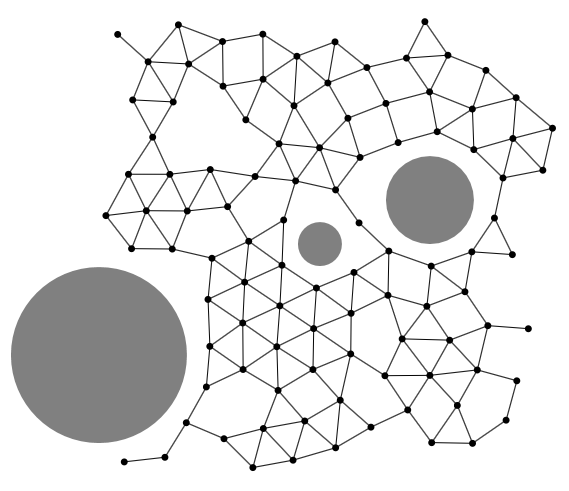
\includegraphics[width=7cm]{obstacles.png}

  \caption{}
  \label{obstacles}

\end{figure}

\section{Conclusion}


\end{multicols}

\bibliographystyle{alpha}
\bibliography{references}

\end{document}
